\documentclass[border=15pt, multi, tikz]{standalone}

\usepackage{tikz}
\usetikzlibrary{quotes,arrows.meta}
\usetikzlibrary{positioning}
\def\edgecolor{rgb:blue,4;red,1;green,4;black,3}
\newcommand{\midarrow}{\tikz \draw[-Stealth,line width =0.8mm,draw=\edgecolor] (-0.3,0) -- ++(0.3,0);}
\usepackage{Box}
\usepackage{RightBandedBox}

\def\ConvColor{rgb:blue,5;green,2.5;white,5}
\def\ConvReluColor{rgb:blue,5;green,5;white,5}
\def\PoolColor{rgb:red,1;black,0.3}
\def\DcnvColor{rgb:blue,5;green,2.5;white,5}
\def\UnpoolColor{rgb:yellow,5;red,2.5;white,5}
\def\SoftmaxColor{rgb:magenta,5;black,7}

\usetikzlibrary{3d} %for including external image 

\begin{document}

\begin{tikzpicture}
\tikzstyle{connection}=[ultra thick,every node/.style={sloped,allow upside down},draw=\edgecolor,opacity=0.7]
%%%%%%%%%%%%%%%%%%%%%%%%%%%%%%%%%%%%%%%%%%%%%%%%%%%%%%%%%%%%%%%%%%%%%%%%%%%%%%%%%%%%%%%%
%% Draw Layer Blocks
%%%%%%%%%%%%%%%%%%%%%%%%%%%%%%%%%%%%%%%%%%%%%%%%%%%%%%%%%%%%%%%%%%%%%%%%%%%%%%%%%%%%%%%%
%%%%%%%%%%   
\node (original) at (13,20,0) {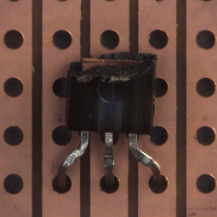
\includegraphics[width=12cm,height=12cm]{img/sub-img/transistor-defective.png}};

\node (mask1) at (0,0,0)  {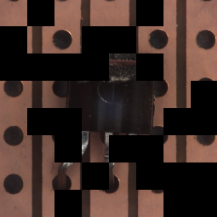
\includegraphics[width=12cm,height=12cm]{img/sub-img/transistor-defective-masked1.png}};
\node (mask2) at (13,0,0) {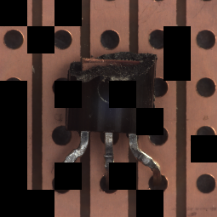
\includegraphics[width=12cm,height=12cm]{img/sub-img/transistor-defective-masked2.png}};
\node (mask3) at (26,0,0) {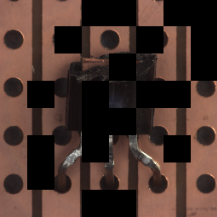
\includegraphics[width=12cm,height=12cm]{img/sub-img/transistor-defective-masked3.png}};


%Connections
\path[->,>=stealth,line width=10pt] (original.south) edge [bend right=10, looseness=1] (mask1.north);
\path[->,>=stealth,line width=10pt] (original.south) edge                              (mask2.north);
\path[->,>=stealth,line width=10pt] (original.south) edge [bend left=10,  looseness=1] (mask3.north);

\end{tikzpicture}
\end{document}\grid
